\par Aqui é apresentada a simulação da trajetória de uma espaçonave que passa pelo ponto (0.1,0) no sistema Terra-Lua. Foram simulados os seguintes casos mostrados na tabela abaixo:

\begin{table}[h]
\centering
\caption{Componentes de Velocidade Relativa}
\label{tab:my-table}
\begin{tabular}{|l|l|l|}
\hline
Caso & $\dot{x}$ & $\dot{y}$ \\ \hline
a)    & 0         & 0.5       \\ \hline
b)    & -4        & 1         \\ \hline
c)    & -3.35     & 3         \\ \hline
d)    & -3.37     & 3         \\ \hline
e)    & -3.4      & 3         \\ \hline
f)    & -3.5      & 3         \\ \hline
g)    & -3.6      & 3         \\ \hline
\end{tabular}
\end{table}


Os resultados obtidos podem ser vistos nas figuras a seguir. Destaca-se que os resultados encontrados ficaram ligeiramente diferentes dos obtidos por \cite{book:226549}. Os autores acreditam que a divergência se dá devido ao solver utilizado. No caso deste trabalho foi utilizado o solver \textit{$solve_{ivp}$} com o método "RK45". Já \cite{book:226549} utiliza o solver ODE45 do \textit{Matlab}.


A trajetória para o caso (a) é simulada com um tempo máximo de t = 1  e é ilustrada na figura \ref{fig: cuzao } abaixo. As órbitas em torno da Terra, com rotação apsidal e nodal do plano orbital causada pela gravidade da lua ficam claras na imagem.

\begin{figure}[H]
\centering
\caption{Caso a}
\label{fig: cuzao}
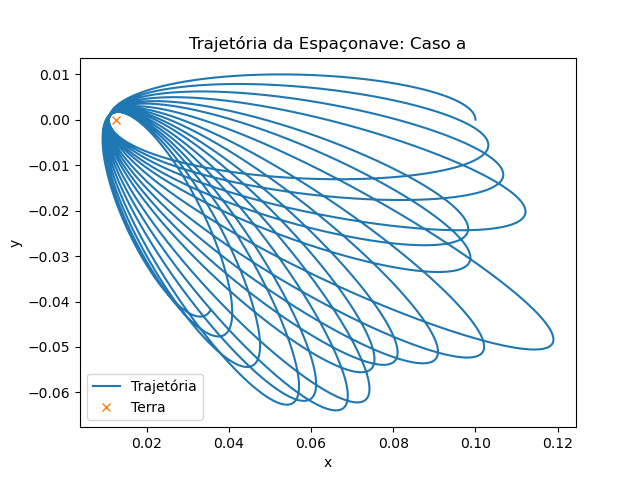
\includegraphics[width=1\textwidth]{figuras/Resultados/7.3/73casoa.png}
\fonte{Autores, 2023}
\end{figure}

\par Com o aumento da velocidade inicial para o caso (b), as órbitas em torno da Terra transformam-se em trajetórias mais energéticas e altamente excêntricas, mesmo assim o veículo  não consegue atravessar o contorno de velocidade zero de C para uma missão lunar. A figura \ref{fig: casobbb} ilustra
o decaimento da órbita com o tempo devido à gravitação da Lua.

\begin{figure}[H]
\centering
\caption{Caso b}
\label{fig: casobbb}
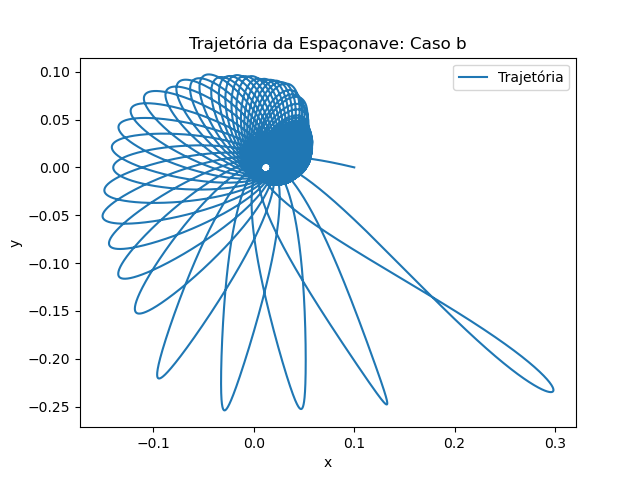
\includegraphics[width=1\textwidth]{figuras/Resultados/7.3/73casob.png}
\fonte{Autores, 2023}
\end{figure}

\par A velocidade inicial do caso (c) é suficientemente grande para uma trajetória de "regresso livre" da Lua para a terra. Neste caso, a nave espacial passa ligeiramente abaixo da órbita da Lua em torno da Terra.

\begin{figure}[H]
\centering
\caption{}
\label{fig: caso c }
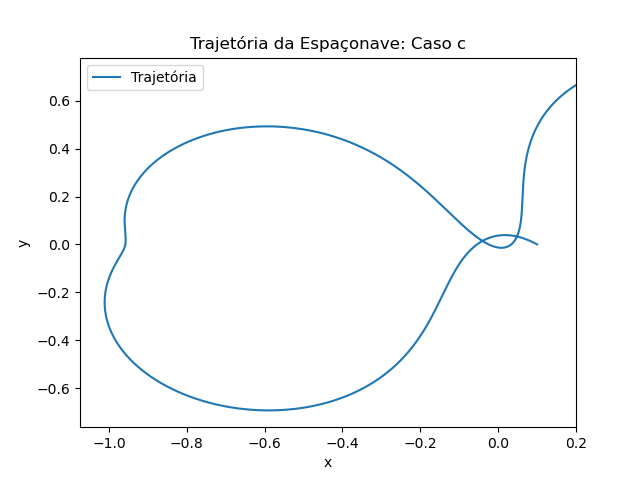
\includegraphics[width=1\textwidth]{figuras/Resultados/7.3/73casoc.png}
\fonte{Autores, 2023}
\end{figure}

\par O tempo total de voo é reduzido significativamente no caso (d) para cerca de t = 2,8, quando a nave espacial passa no entorno da Lua, entre L1 e L2. No processo, a trajetória de regresso tem uma energia cinética ligeiramente maior devido ao impulso dado pelo "estilingue" lunar . As trajetórias lunares de passagem têm sido utilizadas para para impulsionar várias naves espaciais para os pontos lagrangianos sol-terra.

\begin{figure}[H]
\centering
\caption{Caso c}
\label{fig: }
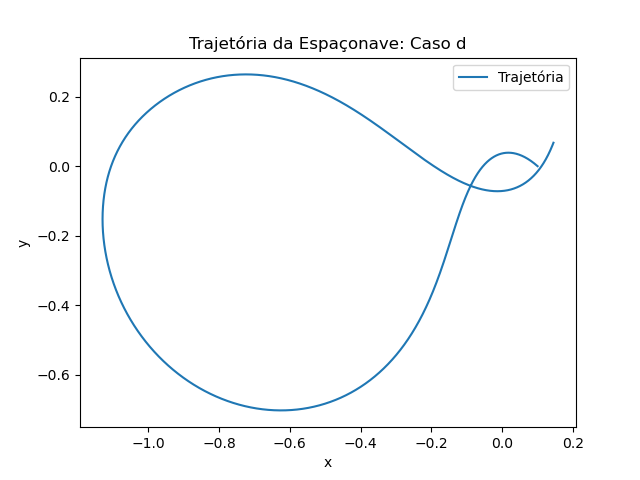
\includegraphics[width=1\textwidth]{figuras/Resultados/7.3/73casod.png}
\fonte{Autores, 2023}
\end{figure}

 No caso (e) , o tempo de voo cresce para cerca de
 t = 3.45 para uma volta completa, uma vez que a espaçonave passa mais longe da lua, passando depois do ponto L1.


\begin{figure}[H]
\centering
\caption{Caso d}
\label{fig: }
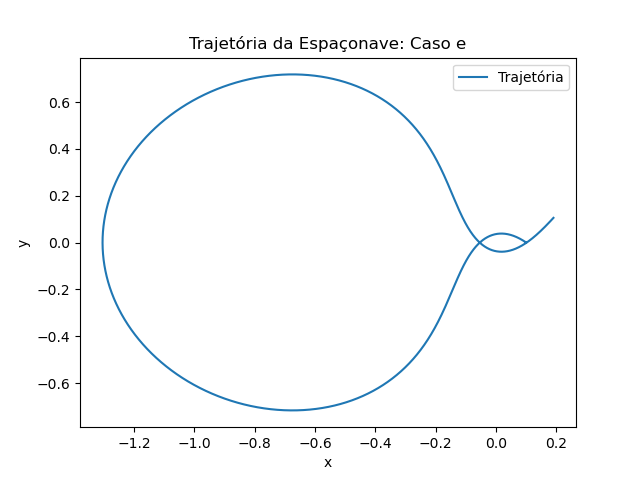
\includegraphics[width=1\textwidth]{figuras/Resultados/7.3/73casoe.png}
\fonte{Autores, 2023}
\end{figure}

Para os casos $f$ e $g$, figuras \ref{fig: f} e \ref{fig: g} respectivamente, há diferenças qualitativas nas trajetórias. é observado que para um longo tempo o caso $f$ demonstra que a espaçonave faz uma passagem pela lua a uma grande distância de $L_1$, porém é incapaz de escapar da gravidade terrestre, fazendo se aproximar mais da lua na próxima passagem, conforme mais passagens ocorrem a espaçonave é trazida para a órbita da terra com um decrescimento do raio. O caso $f$ ilustra um método mais barato para trazer um satélite para uma órbita geossíncrona, através de múltiplas passagens através da lua. Um método similar é encontrado para múltiplas passagens em planetas para diminuir o custo de missões interplanetárias.

Conforme ocorre o aumento da energia inicial para o caso $g$, a espaçonave não retorna para terra e sim embarca em uma trajetória de escape do sistema terra-lua. Nessa trajetória, a vantagem encontra-se na ajuda recebida pela gravidade lunar reduzindo o consumo de combustível e consequentemente o custo de missões interplanetárias.

\begin{figure}[H]
\centering
\caption{Caso f}
\label{fig: f}
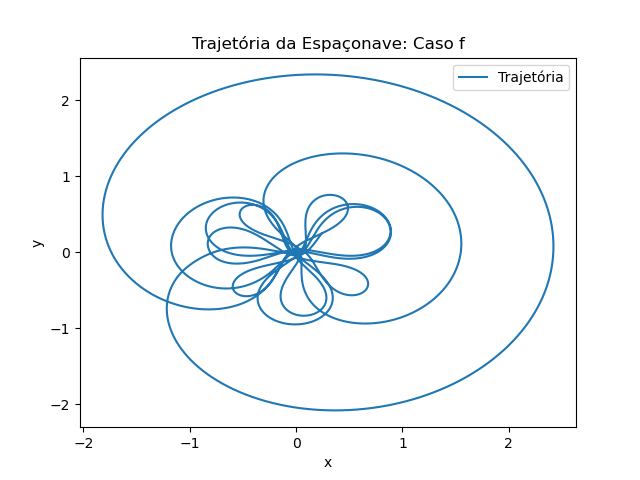
\includegraphics[width=1\textwidth]{figuras/Resultados/7.3/73casof.png}
\fonte{Autores, 2023}
\end{figure}

\begin{figure}[H]
\centering
\caption{Caso g}
\label{fig: g}
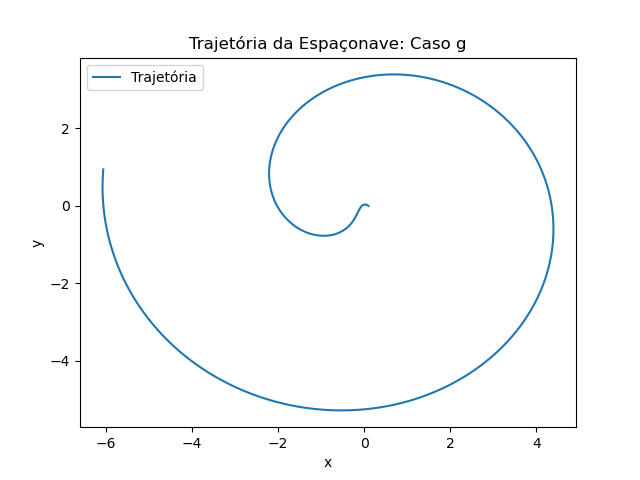
\includegraphics[width=1\textwidth]{figuras/Resultados/7.3/73casog.png}
\fonte{Autores, 2023}
\end{figure}